\documentclass[10pt,a4paper]{article}

\usepackage[utf8]{inputenc}
\usepackage[T1]{fontenc}
\usepackage[brazilian]{babel}
\usepackage{lmodern}
\usepackage{microtype}
\usepackage{geometry}
\usepackage{amsmath}
\usepackage{array}
\usepackage{booktabs}
\usepackage{enumitem}
\usepackage{graphicx}
\usepackage{xcolor}
\usepackage{tikz}
\usetikzlibrary{arrows.meta,positioning,calc}
\usepackage{pgfgantt}
\usepackage{titlesec}
\usepackage{fancyhdr}
\usepackage{setspace}
\usepackage[hidelinks]{hyperref}
\hypersetup{
  pdftitle={Proposta de Trabalho - Contagem e Identificacao Automatica de Resistores em Imagens},
  pdfauthor={Pedro Nicollas Pereira Azevedo Della Torre Bastos}
}

\geometry{a4paper,top=2.0cm,bottom=2.0cm,left=2.2cm,right=2.2cm}
\setstretch{1.04}
\setlength{\parindent}{1.25cm}
\setlength{\parskip}{0.12cm}
\setlist[itemize]{leftmargin=1.25em,itemsep=0.05em,topsep=0.08em}
\renewcommand{\arraystretch}{1.05}
\graphicspath{{proposta_assets/}}

\definecolor{azul}{RGB}{0,0,0}
\definecolor{azulmedio}{RGB}{0,0,0}
\definecolor{azulclaro}{RGB}{255,255,255}
\definecolor{cinza}{RGB}{0,0,0}

\titleformat{\section}{\large\bfseries\color{azul}}{}{0pt}{}
\titlespacing*{\section}{0pt}{0.45em}{0.22em}

\pagestyle{fancy}
\fancyhf{}
\fancyhead[L]{\scriptsize Proposta de trabalho - Processamento de Sinais 2}
\fancyhead[R]{\scriptsize Detecção de resistores}
\fancyfoot[C]{\small\thepage}
\renewcommand{\headrulewidth}{0.3pt}
\renewcommand{\footrulewidth}{0pt}

\begin{document}
\hypersetup{pageanchor=false}

% Capa
\begin{titlepage}
\thispagestyle{empty}
\centering
\vspace*{0.6cm}
{\small\bfseries CENTRO FEDERAL DE EDUCAÇÃO TECNOLÓGICA CELSO SUCKOW DA FONSECA\\[2pt]
CAMPUS MARACANÃ\\[2pt]
ENGENHARIA ELETRÔNICA\\[2pt]
PROCESSAMENTO DE SINAIS 2\\[2pt]
Prof Gabriel Matos Araujo}

\vfill
{\LARGE\bfseries
CONTAGEM E IDENTIFICAÇÃO AUTOMÁTICA\\[4pt]
DO VALOR DE RESISTORES\\[4pt]
EM IMAGENS}

\vfill
{\large Pedro Nicollas Pereira Azevedo Della Torre Bastos}

\vfill
Rio de Janeiro, Rio de Janeiro, Brasil\\[3pt]
Outubro de 2026
\end{titlepage}

\clearpage
\hypersetup{pageanchor=true}
\pagenumbering{arabic}
\setcounter{page}{1}

\section{Introdução e descrição do problema}

Resistores axiais são identificados, em geral, pela sequência de faixas coloridas impressa no corpo do componente. A leitura manual é simples para poucas peças, mas se torna lenta e sujeita a erros quando a imagem contém muitos resistores, diferentes orientações, reflexos, desfoque, variações de iluminação ou cores visualmente próximas.

Este trabalho propõe um sistema de visão computacional capaz de receber imagens estáticas, localizar cada resistor, contar os componentes e informar individualmente o valor da resistência e a tolerância. A saída deverá relacionar cada detecção a uma região da imagem, por exemplo: \textit{R1 - 470~$\Omega$ $\pm$5\%}. O escopo inicial usa aquisição parcialmente controlada com resistores separados; vídeos e fitas com muitos componentes ficam como extensões futuras, caso haja tempo.

\section{Metodologia e proposta de solução}

A solução será implementada como um pipeline híbrido, compatível com Windows e Linux, inspirado principalmente no artigo de Clark Kneil Caoile, \href{https://doi.org/10.5281/zenodo.20699559}{``Automatic Resistor Value Detection Using Computer Vision and Machine Learning''} (\textit{Journal of Engineering and Technology for Sustainability and Resilience}, v. 1, n. 1, p. 10--16, 2026). A ideia central do artigo --- localizar a região de interesse e classificar as faixas --- será ampliada para vários componentes separados na mesma imagem. Após a aquisição, serão comparados correção de iluminação, redução de ruído e análise em RGB, HSV e CIELAB, além de métodos clássicos (limiarização, segmentação, morfologia e contornos) e modelos aprendidos, como YOLO. As abordagens do detector MATLAB e do Automatic Component Analyzer serão usadas como referências complementares no benchmark.

Cada detecção será recortada e alinhada pelo eixo do resistor. As faixas serão analisadas por perfis de cor e classificadores complementares; em seguida, o código de cores será convertido em ohms e tolerância. Como extensão futura, para vídeos, o mesmo componente poderá ser rastreado entre quadros e as evidências fundidas temporalmente, reduzindo o efeito de um frame desfocado. O benchmark separará contagem, localização, leitura das faixas e resultado final.

\begin{center}
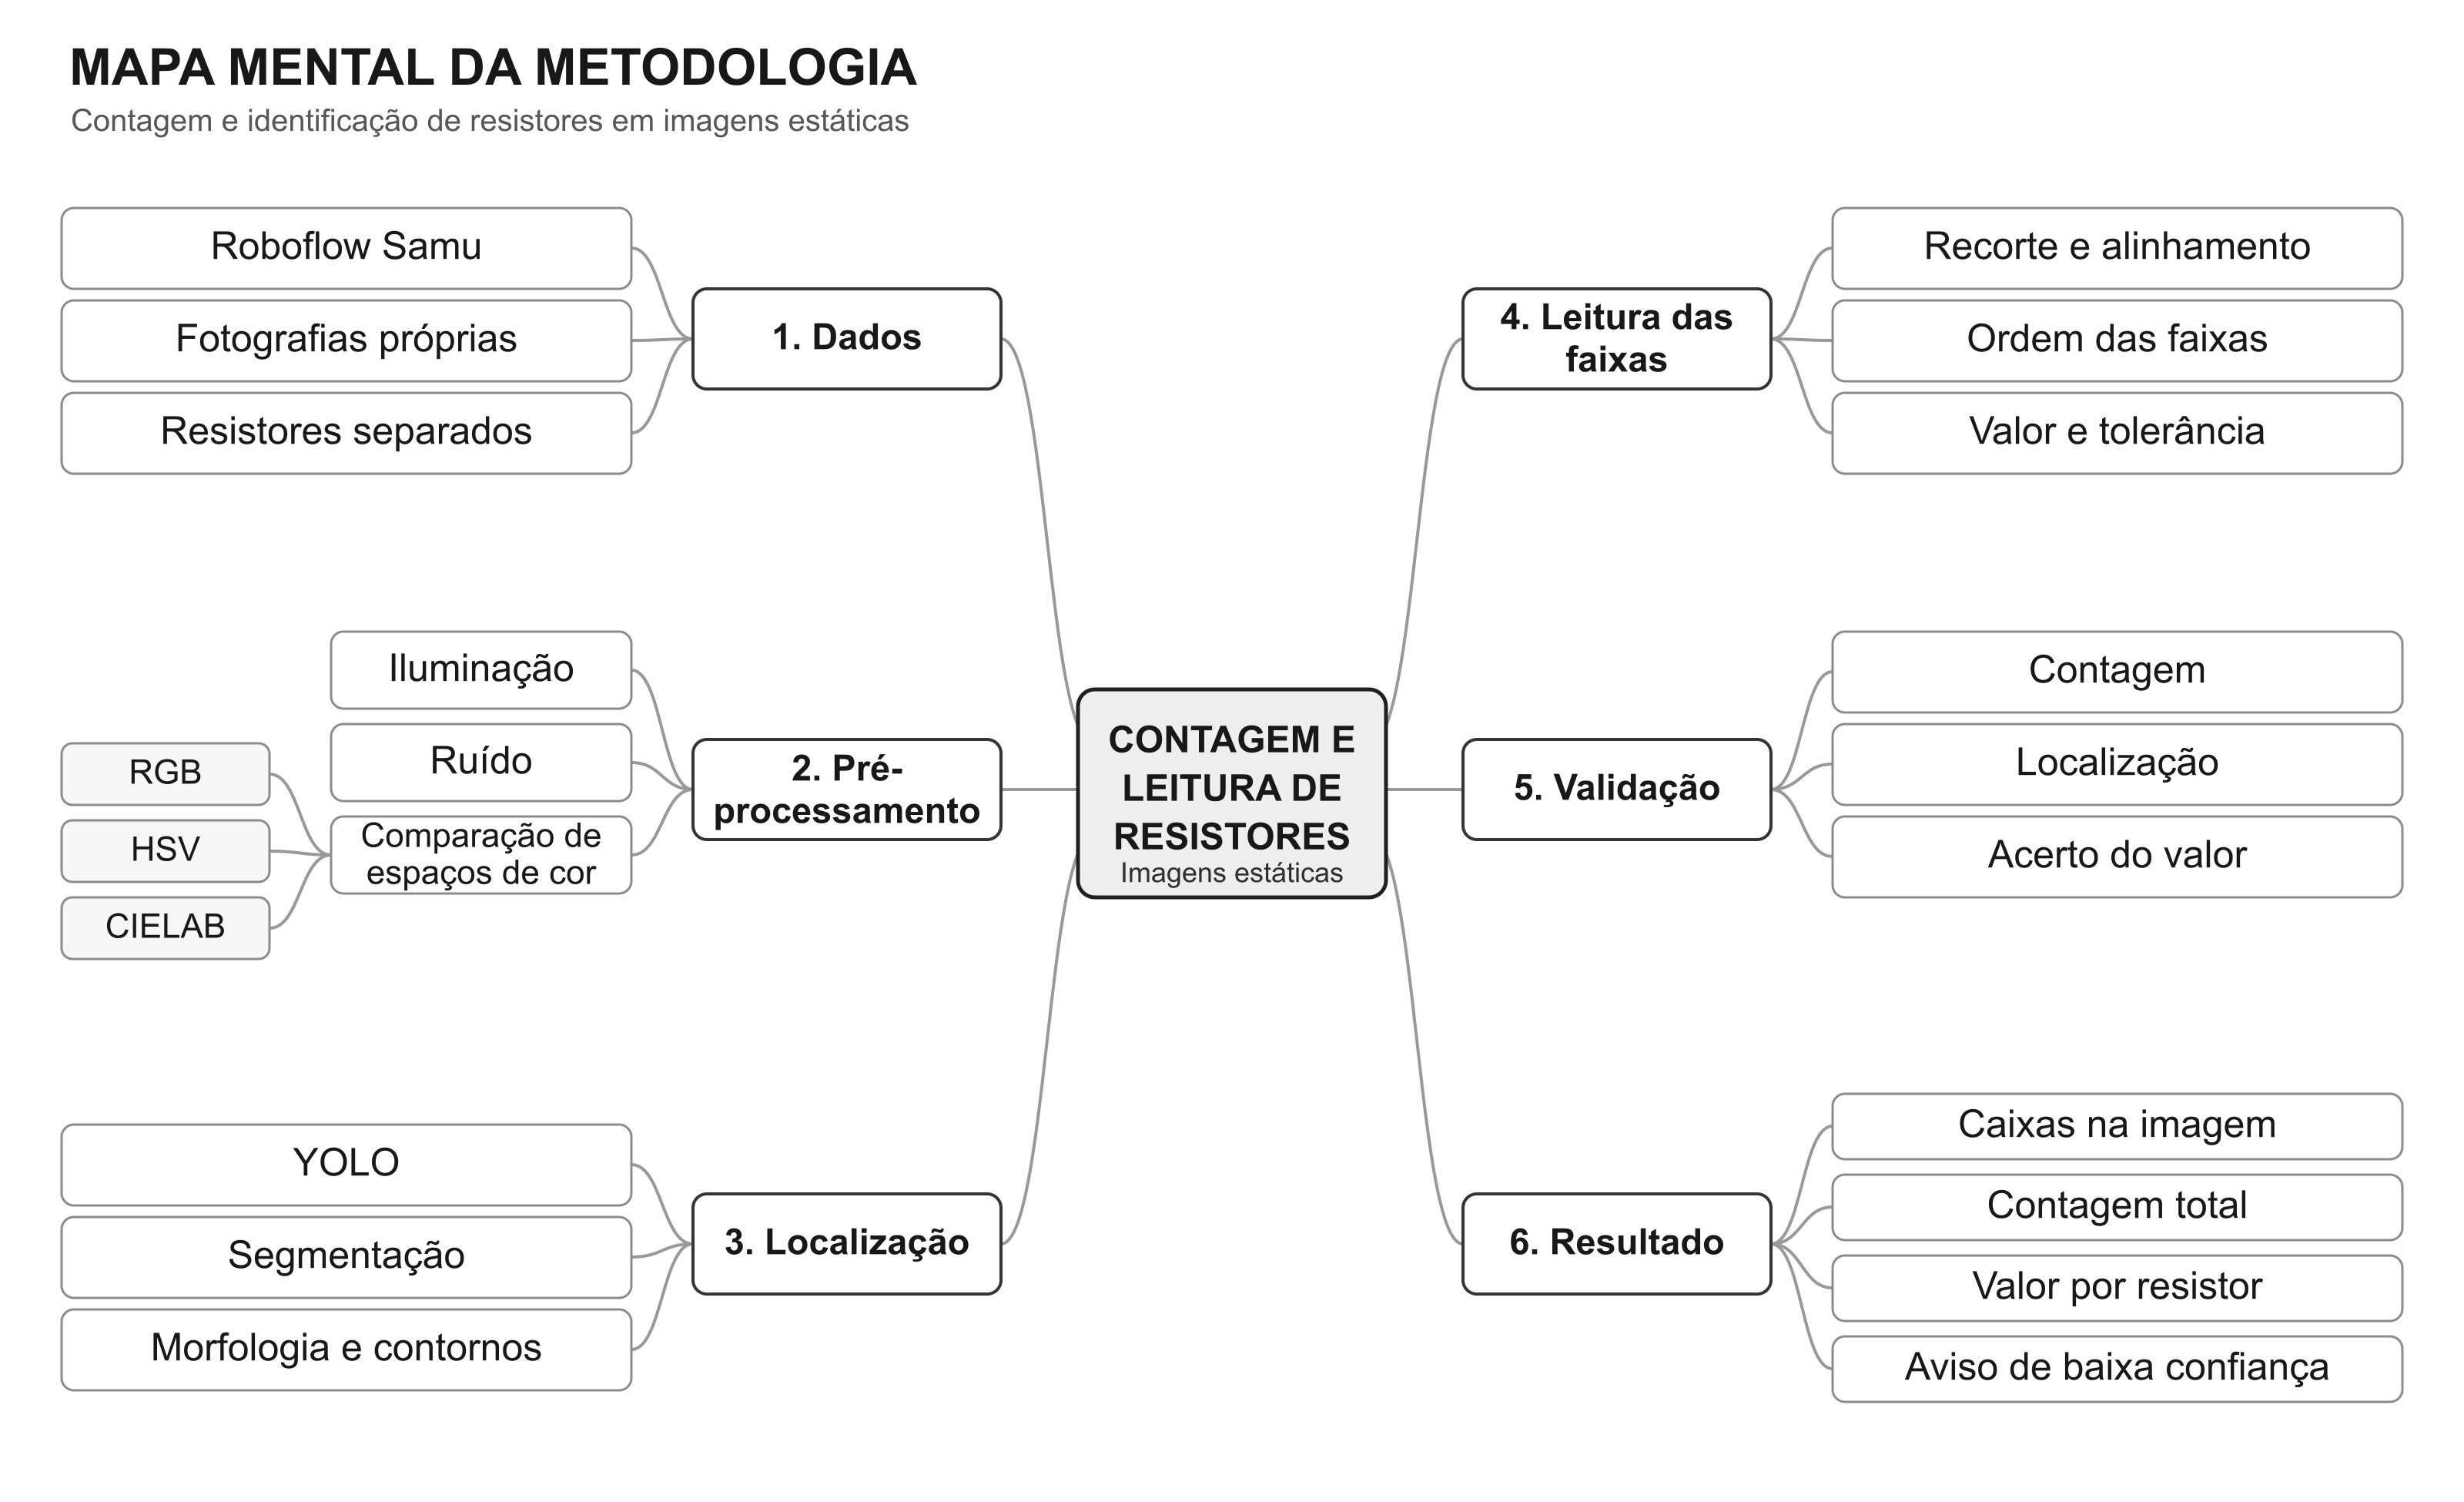
\includegraphics[width=0.98\textwidth]{mapa_mental_resistores_previa.png}
\end{center}
\clearpage

\section{Descrição do dataset}

O dataset principal será o export YOLO do Roboflow Samu, denominado \texttt{electronic-components-d6uul}. Ele será a referência para detecção e contagem, pois reúne 9.850 imagens e 2.794 registros de resistores no manifesto utilizado no projeto. O conjunto próprio incluirá fotografias com um ou vários resistores separados, diferentes posições, rotações, distâncias, fundos e condições de iluminação.

Serão organizadas três camadas de anotação:
\begin{itemize}
    \item caixas delimitadoras ou máscaras para localizar cada resistor;
    \item sequência de cores, orientação e valor nominal para treinar/validar a leitura;
    \item identidade do componente entre frames, caso a extensão para vídeo seja realizada.
\end{itemize}

Os dados serão separados por imagem, cena e conjunto de componentes, evitando que recortes quase idênticos apareçam em treino e teste. A divisão inicial será aproximadamente 70\% para treinamento, 15\% para validação e 15\% para teste, com aumento de dados para variações de iluminação, ruído, rotação e desfoque.

Outros datasets serão usados apenas quando necessário para complementar o principal: Alptugaydin para máscaras de segmentação, Barrettotte para bandas e valores, Eralp Ozcan, MathWorks, Zenodo e outros exports Roboflow para variações de cena e validação externa. As imagens de fitas com componentes repetidos poderão ser avaliadas como extensão futura para contagem em alta densidade.

\begin{center}
\vspace{-0.2cm}
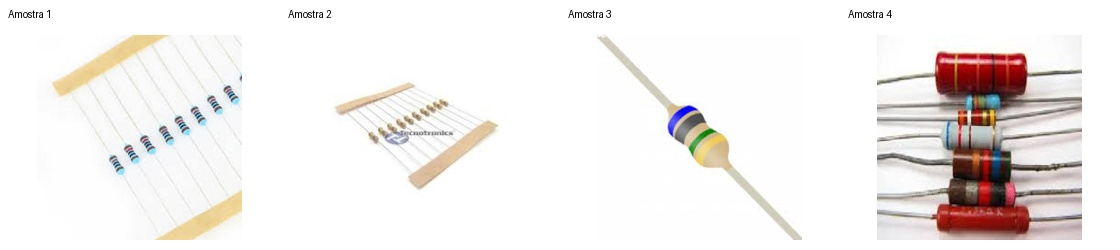
\includegraphics[width=0.68\textwidth]{dataset_examples_strip.jpg}\\[-1pt]
{\scriptsize Exemplos de imagens do dataset principal (Roboflow Samu)}
\end{center}

\section{Resultados esperados}

Espera-se obter uma aplicação que, para cada imagem, apresente a quantidade de resistores e uma lista individual com caixa, valor em ohms, tolerância e confiança. Para vídeos, como extensão futura, espera-se uma leitura estável ao longo dos quadros. O desempenho será medido por:
\begin{itemize}
    \item contagem exata e erro absoluto de contagem;
    \item precisão, \textit{recall} e mAP para localização;
    \item acurácia do valor nominal e da tolerância, incluindo acerto dentro da tolerância esperada;
    \item tempo de processamento por imagem.
\end{itemize}

A meta inicial é superar 95\% de contagem exata em cenas controladas e obter leitura correta na maioria dos recortes legíveis, sem forçar um valor quando as faixas estiverem ocultas ou ambíguas. Nesses casos, o sistema deverá indicar baixa confiança para permitir revisão humana.

\section{Cronograma}

O desenvolvimento será incremental, começando pela organização dos dados e pela contagem, depois incorporando a leitura das faixas, a integração e a avaliação final.

\begin{center}
\resizebox{0.72\textwidth}{!}{%
\begin{ganttchart}[
    hgrid, vgrid,
    x unit=0.64cm,
    y unit chart=0.28cm,
    title height=0.7,
    bar height=0.24,
    title label font=\bfseries\scriptsize,
    bar label font=\scriptsize,
    bar label node/.append style={align=right},
    bar/.append style={fill=azulclaro, draw=azulmedio},
    group/.append style={fill=azul, draw=azul}
]{1}{8}
\gantttitle{Semanas}{8}\\
\gantttitlelist{1,...,8}{1}\\
\ganttbar{Pesquisa e requisitos}{1}{2}\\
\ganttbar{Dataset e anotações}{1}{3}\\
\ganttbar{Pré-processamento}{2}{4}\\
\ganttbar{Detecção e contagem}{3}{5}\\
\ganttbar{Faixas e valor}{5}{6}\\
\ganttbar{Integração}{6}{7}\\
\ganttbar{Benchmark e ajustes}{7}{8}\\
\ganttbar{Relatório e apresentação}{7}{8}
\end{ganttchart}%
}
\end{center}

\end{document}
